\chapter{The Standard Model, Higgs Boson and New Scalar Particles }

\section{The Standard Model}

\section{The Higgs Boson}

\section{New Scalar Particles}

There are many deficiencies of the Standard Model (SM), such as the hierarchy problem,
flavor problem, dark matter problem, cosmological constant problem, electroweak symmetry breaking problem, CP violation problem, baryogenesis problem, etc.
The presence of a hidden sector, defined here to mean extra states that
have no SM gauge charge but are charged under some other exotic gauge symmetry, does not necessarily solve any of the problems above. However, in order to identify whether the SM Higgs sector is complete,  the searches of additional heavy scalars are performed.  They would prove the presence of beyond-the-SM (BSM) physics in the form of a non-minimal Higgs sector~\cite{Robens:2015gla}. The existence of sibling Higgs boson, denoted X, is motivated in many BSM scenarios, so the research in the full mass range accessible at colliders  remains one of the main objectives of the experimental community. This  road  needs  to  be continued within the full mass range that is accessible to current and future experiments.
\newline
\subsection*{Higgs Singlet Extension}
The simplest extension of the SM Higgs sector consist in an additional singlet which is neutral under all quantum number of the SM gauge groups.
A complex $SU(2)_L$ doublet,  denoted $\Phi$, is added by an additional real scalar $S$ which is a singlet under all SM gauge groups. 
The most general gauge-invariant and renormalisable scalar Lagrangian is,


\begin{equation}
 \mathcal{L}_s = (D_{\mu} \Phi )^{\dagger}  \: D_{\mu} \Phi  +  \partial^{\mu}S   \partial_{\mu}S -V(\Phi, S)     \end{equation}
where $V(\Phi, S) $ is the scalar potential,  

\begin{equation}
 V(\Phi, S)= -m^2   \Phi ^{\dagger}\Phi -\mu^2 S^2 +\lambda_1 (\Phi ^{\dagger}\Phi)^2 +\lambda_2 S^4 + \lambda_3 \Phi ^{\dagger}\Phi^2 S^2  \end{equation}
Here, $Z_2$ ($S \rightarrow -S$) symmetry is imposed which forbids additional terms in the potential.
The scalar potential $V(\Phi, S)$ is bounded from below if the following conditions are fulfilled,

\begin{equation}
 4 \lambda_1  \lambda_2 - \lambda_3^2 >0    \end{equation}

\begin{equation}
 \lambda_1 , \lambda_2  >0    \end{equation}

where if the first condition is fulfilled, the extremum is a local minimum. The
second condition (5), guarantees that the potential is bounded from below for large field values.
The Higgs fields, $\Phi$ and $S$, have non-zero vacuum expectation, denoted by $v$ and $x$, respectively.
Following the unitary-gauge prescription, the the Higgs fields is given by,
\newline
$$
{\mathcal H} \equiv \left(
\begin{array}{c}
0  \\
\frac{\tilde{h}+v }{\sqrt{2}}  \\
\end{array}
\right)
, \qquad 
S \equiv \frac{h'+x }{\sqrt{2}}
.
$$
Expansion around the minimum leads to the squared mass matrix
\newline
$$
{\mathcal M}^2 = \left(
\begin{array}{cc}
2 \lambda_1^2 v^2 & \lambda_3 vx  \\
\lambda_3 vx & 2 \lambda_1^2 x^2 \\

\end{array}
\right)
$$
\newline
with the mass eigenvalues

\begin{equation}
 m_h^2=  \lambda_1 v^2 + \lambda_2 x^2 -\sqrt{(\lambda_1 v^2 - \lambda_2 x^2)^2 +\lambda_3 (xv)^2 } \qquad,  \end{equation}

\begin{equation}
 m_H^2=  \lambda_1 v^2 + \lambda_2 x^2 +\sqrt{(\lambda_1 v^2 - \lambda_2 x^2)^2 +\lambda_3 (xv)^2 } \qquad,  \end{equation}
\newline
where $h$ and $H$ are the scalar fields of definite masses $m_h$ and $m_H$ respectively, with $m_h^2 < m_H^2$ .
The gauge and mass eigenstates are related via the mixing matrix
\newline
$$
\left(
\begin{array}{c}
h   \\
H \\
\end{array}
\right)
=
\left(
\begin{array}{cc}
\cos \alpha & -\sin \alpha   \\
\sin \alpha & \cos \alpha \\
\end{array}
\right)
\;
\left(
\begin{array}{c}
\tilde{h}   \\
h' \\
\end{array}
\right)
$$
\newline
where the mixing angle $ - \frac{\pi}{2} \leq \alpha \leq  \frac{\pi}{2} $ is given by,
\newline
\begin{equation}
\sin 2 \alpha= \frac{\lambda_3 xv}{\sqrt{(\lambda_1 v^2 - \lambda_2 x^2)^2 +\lambda_3 (xv)^2 } } \; , \end{equation}


\begin{equation}
\cos 2 \alpha= \frac{\lambda_2 x^2 - \lambda_1 v^2}{\sqrt{(\lambda_1 v^2 - \lambda_2 x^2)^2 +\lambda_3 (xv)^2 } } \; .  \end{equation}
\newline
By the  mixing matrix it is clear that the light (heavy) Higgs couplings to SM particles are now
suppressed by $\cos \alpha $ ( $\sin \alpha $).
The heavy Higgs is a new version of the SM Higgs with rescaled couplings
to the matter contents and to the gauge fields of the SM. In fact, the only novel channel
with respect to the light Higgs case is $H \rightarrow hh$. The partial decay width $\Gamma$ is given by \cite{Schabinger:2005ei},
\newline
\newline
 \begin{equation}
\Gamma_{ H \rightarrow hh} =  \frac{|\mu'|^2}{8 \pi m_H } \, \sqrt{1- \frac{4m_h^2}{m_H^2}}  \; , \end{equation}
\newline
where the coupling strength $\mu'$ is,
\newline
\begin{equation}
 \mu' =  - \frac{\sin 2 \alpha}{2vx} \, (\sin \alpha v + \cos \alpha x) \, (m_h^2 + \frac{m_H^2}{2})  \; . \end{equation}
\newline
In collider phenomenology, is important:
\begin{itemize}
\item the suppression of the production cross section of the two Higgs states induced by the mixing
\item the suppression of the Higgs decay modes to SM particles,
\end{itemize}
For the high mass  scenario, i.e. the case where the heavy Higgs boson is identified with the discovered Higgs state at $\sim$125 GeV, $|\sin \alpha| $= 1 corresponds to the complete decoupling of the second Higgs boson and therefore the SM-like scenario.


\subsection*{Minimal Supersymmetric Standard Model} The simplest extension to the SM, which provides a
framework addressing naturalness, gauge coupling unification, and the existence of
dark matter, is the Minimal Supersymmetric Standard Model (MSSM)~\cite{FAYET1976159}.
Theories where two Higgs fields transform as doublets under $SU(2)_L$ with unit charge $U(1)_Y$, are very interesting. 
The Two Higgs Double Models (2HDMs)~\cite{Barroso:2013zxa} are models that provide
a general effective theory framework for extensions of the electroweak symmetry
breaking sector. In the 2HDMs models, after the EW  symmetry breaking five physical Higgs  particles emerging: 
two neutral CP-even scalars, h, H; one neutral, CP-odd pseudoscalar, A; and two charged scalars, H$^{+}$ and H$^{-}$. All these particles are expected to have a mass at the TeV scale, so in a regime accessible to the particle colliders, as LHC.
The mass spectrum could be divided  in two regions scale: a light Higgs-like particle (h) with mass $m_h= 125$ GeV, and four remaining scalar particle $H$, $A$, $H*{\pm}$, with higher mass and with $m_H \sim m_A \sim m_{H^{\pm}}$.
The Yukawa coupling, in the model with only two Higgs doublets $\Phi_{1,2}$ are~cite{Craig:2012pu},
 \begin{equation}
V_{Yukawa}= - \sum_{i=1,2} (Q \tilde{\Phi_i} \, y_i^{u^{-}}  \bar{u} \, + Q \Phi_i \, y_i^{d} \, \bar{d} + L \Phi_i \, y_i^{e^{-}} e \, + h.c.  )   \; , \end{equation}
where
by convention up-type quarks are always taken to couple to $\Phi_2^0$.
The Glashow-Weinberg condition, that all fermions of a given representation receive their masses through renormalizable
Yukawa couplings, is satisfied by:
\begin{itemize}
\item Type 1, where $y_1^{u,d,e}=0$  (all fermions couple to one doublet).
\item Type 2, where $y_1^u=y_2^d= y_2^e$=0 (the up quark couple to one doublet and the down quarks and leptons couple to the other).
\item Type 3, where $y_1^u=y_1^d= y_2^e$=0 (quarks couple to one doublet and leptons to the other).
\item Type 4, where $y_1^u=y_1^d= y_1^e$=0 (up quark and leptons couple to one doublet and down quarks couple to the other.)
\end{itemize}
Free parameters of the theory are the masses of the  $H$, $A$, $H*{\pm}$ scalars and the angles $\alpha$, $\beta$ that  ully determine the couplings between a single physical Higgs boson and two gauge bosons or two fermions, as well as the coupling between two Higg and a single gauge boson:
\begin{itemize}
\item $\tan \beta =| \Phi_2^0 / \Phi_1^0|$, (expectation value of the ratio among $\Phi_{1,2}^0$).
\item $\alpha$ that is the mixing angle that diagonalizes the $h-H$ mass squared matrix.
\item The four $m_{h,H,A,H^{\pm}}$ masses. 
\end{itemize}
The  wide  range  of  possibilities  for  Higgs  boson  mass  spectrum  hierarchies  and  branching
ratios  in  2HDMs  yields  a  diversity  of  production  and  decay  channels  that  are  relevant  for
multi-lepton  signatures  at  the  LHC.  Multi-lepton  final  states  become  especially  important
when the decay of one Higgs scalar to a pair of Higgs scalars or a Higgs scalar and a vector
boson is possible.  


\subsection*{The $WW$ channel for high mass particle}
Let’s now concentrate on the $X \to WW$ channel, that is the main final state described in the following in the high mass searches.
The two dominant production mechanisms of high mass SM-like Higgs boson are the
gluon gluon fusion and vector boson fusion (VBF) Fig. \ref{prod}. 
The first one is the main mechanism for mass values below 1 TeV, above the VBF production mechanism become more and more important as $m_X$ approaches to high values.
\begin{figure}
\centering
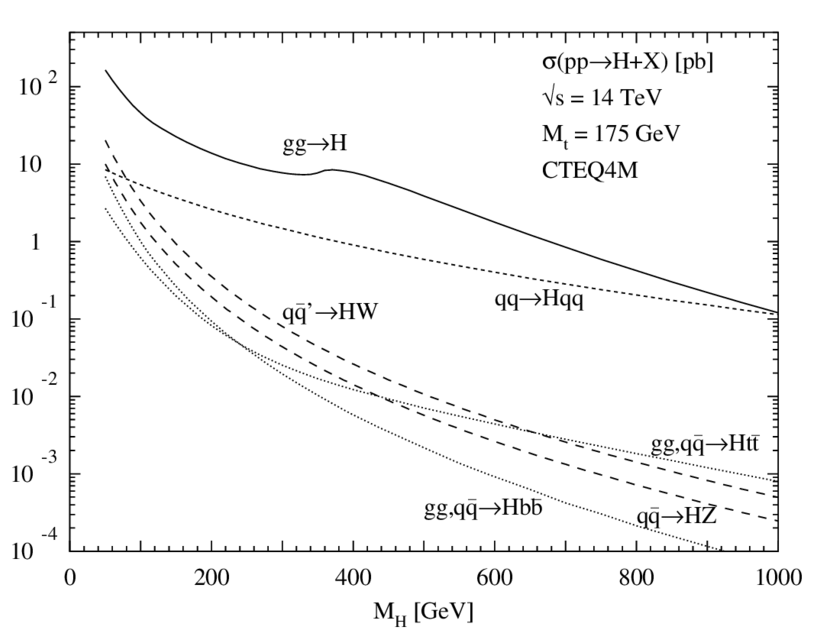
\includegraphics[scale= 0.3]{../Cap1/Higgs-production-cross-sections-at-the-LHC-for-various-production-mechanisms-as-a}
\caption{Higgs-production cross sections at the LHC for various production mechanisms as a function of the Higgs mass. QCD corrections are included except for Higgs bremsstrahlung~\cite{Djouadi2004}.}
\label{prod}
\end{figure}
In the search of high mass Higgs boson for different models scenario, the WW final state, along with ZZ, is the dominant decay channel of $X$ for masses above $2m_Z$ threshold. This fact is evident in Fig. \ref{br} (a), where the $WW$ branching (in green) ratio is dominated in the high mass spectrum. More detailed results on the decays $H \to WW$ and $H \to ZZ $ with the subsequent decay are presented in Fig. \ref{br} (b).
However the yield for the decay channels started by the $X \to WW$ decay is even higher, but the
presence of neutrinos in the final state does not allow to have a completely reconstructed
final state. This fact makes the channel hard to study. 
The gluon gluon fusion production mechanism is characterised by two lepton and two neutrinos in addition to zero or more jets coming from initial state radiation or final state radiation, Sec.~\ref{ps}. The gluon gluon fusion  cross section is between one
and two orders of magnitude larger than that of VBF for a wide range of Higgs masses. Nevertheless, the VBF becomes competitive when the mass approaches to 1 TeV. 
The VBF production, providing two more jets (the VBF jets coming from the hadronization quarks from production) to the final
state, benefits from a highly reduced background with respect to the gluon gluon production mode,
such that even if the VBF production mechanism has a branching ratio smaller than the
gluon-gluon fusion, a higher signal-to-noise ratio is expected.
\begin{figure}
\centering%
\subfigure[]%
{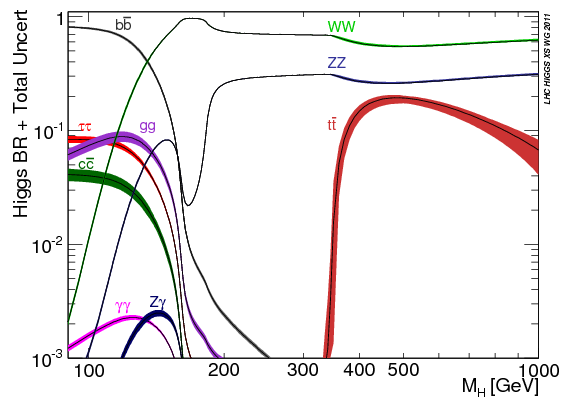
\includegraphics[scale= 0.35]{../Cap1/plots_decay}}
\subfigure[]%
{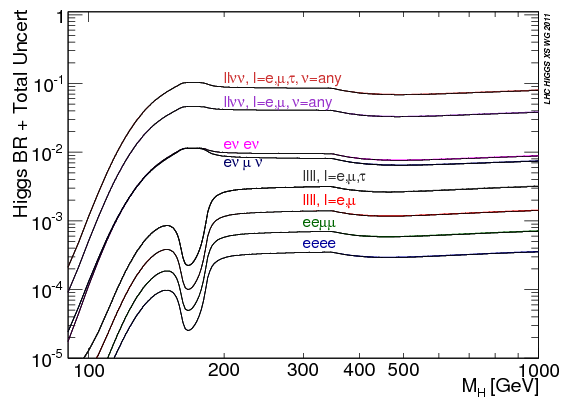
\includegraphics[scale= 0.35]{../Cap1/BRTotalUncertBands4f}}
\caption{(a) Higgs branching ratios and their uncertainties for the full mass range~\cite{Denner:2011mq}. (b) Higgs branching ratios for the different $H \to 4 \ell$ and $H \to 2\ell 2\nu $ final states and their uncertainties for the full mass range~\cite{Denner:2011mq}.}
\label{br}
\end{figure}



\subsection*{$X \to WW$ searches at colliders}
The search of high mass particle with  $WW$ final state  has been widely performed at experiments at hadron
colliders to search for new particles beyond the SM. 
The resonant $WW$ production has been studied at both the Fermilab Tevatron Collider, and the CERN Large
Hadron Collider, with the progressively increasing energy collision and integrated
luminosity. Each machine in its time has therefore probed the highest masses of
 resonances accessible. A review of the different searches
performed by D0, CDF, ATLAS and CMS, their techniques, data, results, and
limits on new particles decaying to $WW$ are described. 

\paragraph{Searches at Tevatron} Before the Higgs boson discovery, the mass  searches for the high masses SM-like Higgs boson has been performed at the CDF
and D0 detector, being the High boson mass a free parameter. 
These searches result in exclusions across the high mass range of 156.5 $<m_H<$173.7 GeV for CDF and 161$<m_H<$170 GeV for D0~\cite{Petridis:2012jd}. 
The high mass searches at CDF and D0 require at least one electron or a muon in the final state in order to suppress the QCD background. Given this requirement all possible decay  modes  are  considered  to  maximise  the  signal  acceptance. The di-lepton plus missing transvere energy channel requires two electrons or muons (plus neutrinos) of opposite charge in the final state. This represents a small WW decay branching ratio, but a clean signature offering the highest sensitivity  of  all  the  high  mass  channels. 
CDF and D0 set limits by combining all of the SM high mass channels with up to 8.2 fb$^{-1}$of integrated luminosity, Fig~\ref{tevatron}.

\begin{figure}
\centering
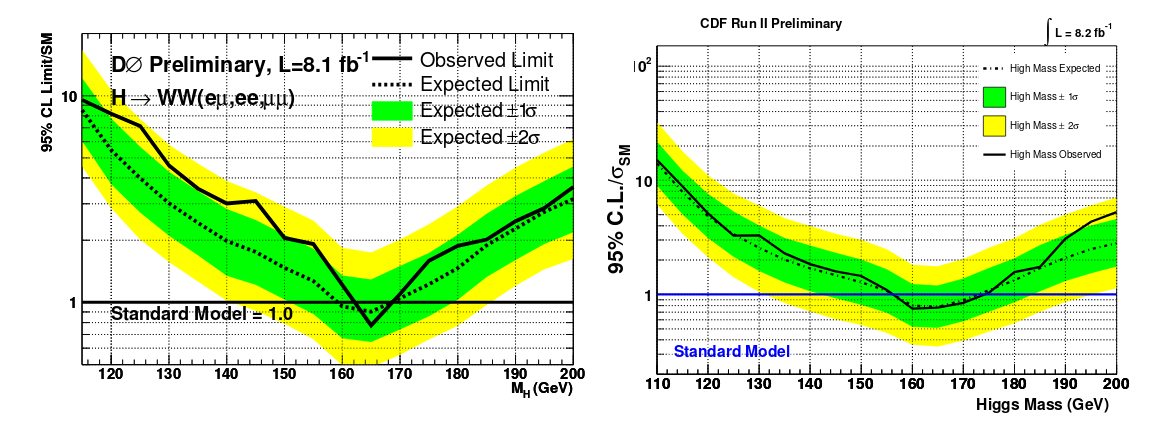
\includegraphics[scale= 0.33]{../Cap1/tevatron}
\caption{Combined limits using the di-lepton channels for D0 (left) and CDF (right).}
\label{tevatron}
\end{figure}

\paragraph{Searches at LHC}

